
% Introduce the different experiments
% If experiment refer to each other, possibly also mention that here.

\chapter{Results \& Discussion}
The experiments performed during the project have led to many interesting results. Each experiment has contributed to improving the system. Either by highlighting issues in the training process or by providing a way to evaluate modelling decisions. 

This chapter presents and discusses the results achieved during the project. The chapter is divided into sections by experiments performed. Each section presents and discusses the results of an experiment. The sections also introduce how the results relate to each other. The order in which these results are presented follows the order in which conclusions were drawn and the project progressed.
% ----------------------------------------------------------------------------------------
% Refer to the description in method
% Present the results of the experiment
    % - What did it do?
    % - Fitness
    % - Generations required before results
    % - (Population)
% Analyse the results and the meanings behind them.
    % - Was it a good result? Why/Why not?
    % - What conclusions can be drawn from the results?
    % - How could we modify this experiment in order to get additional meaningful results?
% ----------------------------------------------------------------------------------------

% refer to the description in Method
% example: did it help to help in any way
% example: present data
% example: did the hypothesis work
\section{Steering a Car Moving at a Constant Speed}
% Här presenteras resultaten för experimenten där hastigheten var fixed
% först utan kurvdata sedan med
% eventuellt någonting om shortest path

As explained in \ref{method:constant_speed}, two experiments where the car moved at a constant speed were conducted during the project. The following sections presents the results achieved during these experiments. Section \ref{subsec:local_perception} presents the behaviour of a system that is not presented with information about the curvature, while section \ref{subsec:fixedspeedcurvature} presents the behaviour of a system that is, as well as a comparison between the two results. Additionally, an observation made when removing the limitations of the cars turning radius is presented in section \ref{sec:shortest}. 

\subsection{Only Local Perception}
\label{subsec:local_perception}
Providing the system only with local perception and giving it control of the steering, as explained in \ref{method:constant_speed}, present interesting results. The system immediately learns that positioning the car in the middle of the track at all times is preferable. Given that the system only has knowledge about the local relation between the car and the track, this behaviour is reasonable.

On straights, this behaviour works well, it could even be considered effective in some scenarios. However, in corners it is not as effective. When the track turns the car will drift away from the middle line. The system responds by steering back toward the middle. Before the system have had sufficient training, the amount of steering is either to large or too small. If the AI steers too much, the car will cross the middle line, and then have to react to that by steering the other way. This leads to the car moving in a sinusoidal pattern along the track, which eventually causes the car to crash. To small of an adjustment instead results in the car not getting back to the middle, which also eventually leads to a crash. It has been observed that moving in a sinusoidal pattern occasionally helps the car to complete a complicated corner, by positioning the car in a good way. Even though this behaviour improves fitness, and in theory could make the car complete the lap with a higher constant speed, it is not an effective or optimal behaviour, thus it is not the target behaviour.

The amount of training required to complete a lap, if possible, is dependent on the constant speed of the car as seen in table \ref{tab:localdata}. When the car manages to complete a lap, the sinusoidal patterns stops due to the amount of steering applied being finely tuned to stay as close to the middle as possible. For speeds higher than $11.7$ m/s, the system never manages to complete a lap. This is due to the cars turning radius being too large to complete every corner by staying to the tracks middle line. Some degree of sinusoidal patterns is beneficial in these scenarios, since they occasionally cause the allowed turning radius through a corner to be larger.

\begin{table}[h!] 
  \centering
  \begin{tabular}{rr}
    \toprule
    Speed [m/s] & Generations\\
    \midrule
    $10.0$ & $2$ \\
    $11.6$ & $5$ \\
    $11.7$ & $22$ \\
    \bottomrule
  \end{tabular}
  \caption{Data of how many generations required until a genome with a constant speed could take a complete lap with local perception.}
  \label{tab:localdata}
\end{table}

\noindent
These results confirm that NEAT can find behaviours that are applicable to steering a race car. The system managed the task better than expected. However, due to the limited information, the system is unable to prepare for an approaching corner in a sophisticated way. The only information the AI can base its decisions on is its current position on the track. Providing information about how the track will progress should enable the system to prepare for upcoming corners. 


\subsection{Local Perception and Track Curvature}
\label{subsec:fixedspeedcurvature}

When using the track curvature data in addition to the local perception, solutions that completed the track was found up to 12.1 m/s. It is 0.4 m/s more than was found not using the curvature data. The difference in speed may seem small, but the difference in behaviour is substantial.

What the solutions found generally do is that they position themselves well before a curve, to compensate for the larger turning radius required. They also start to steer before the curve actually start.

\begin{figure}[H]
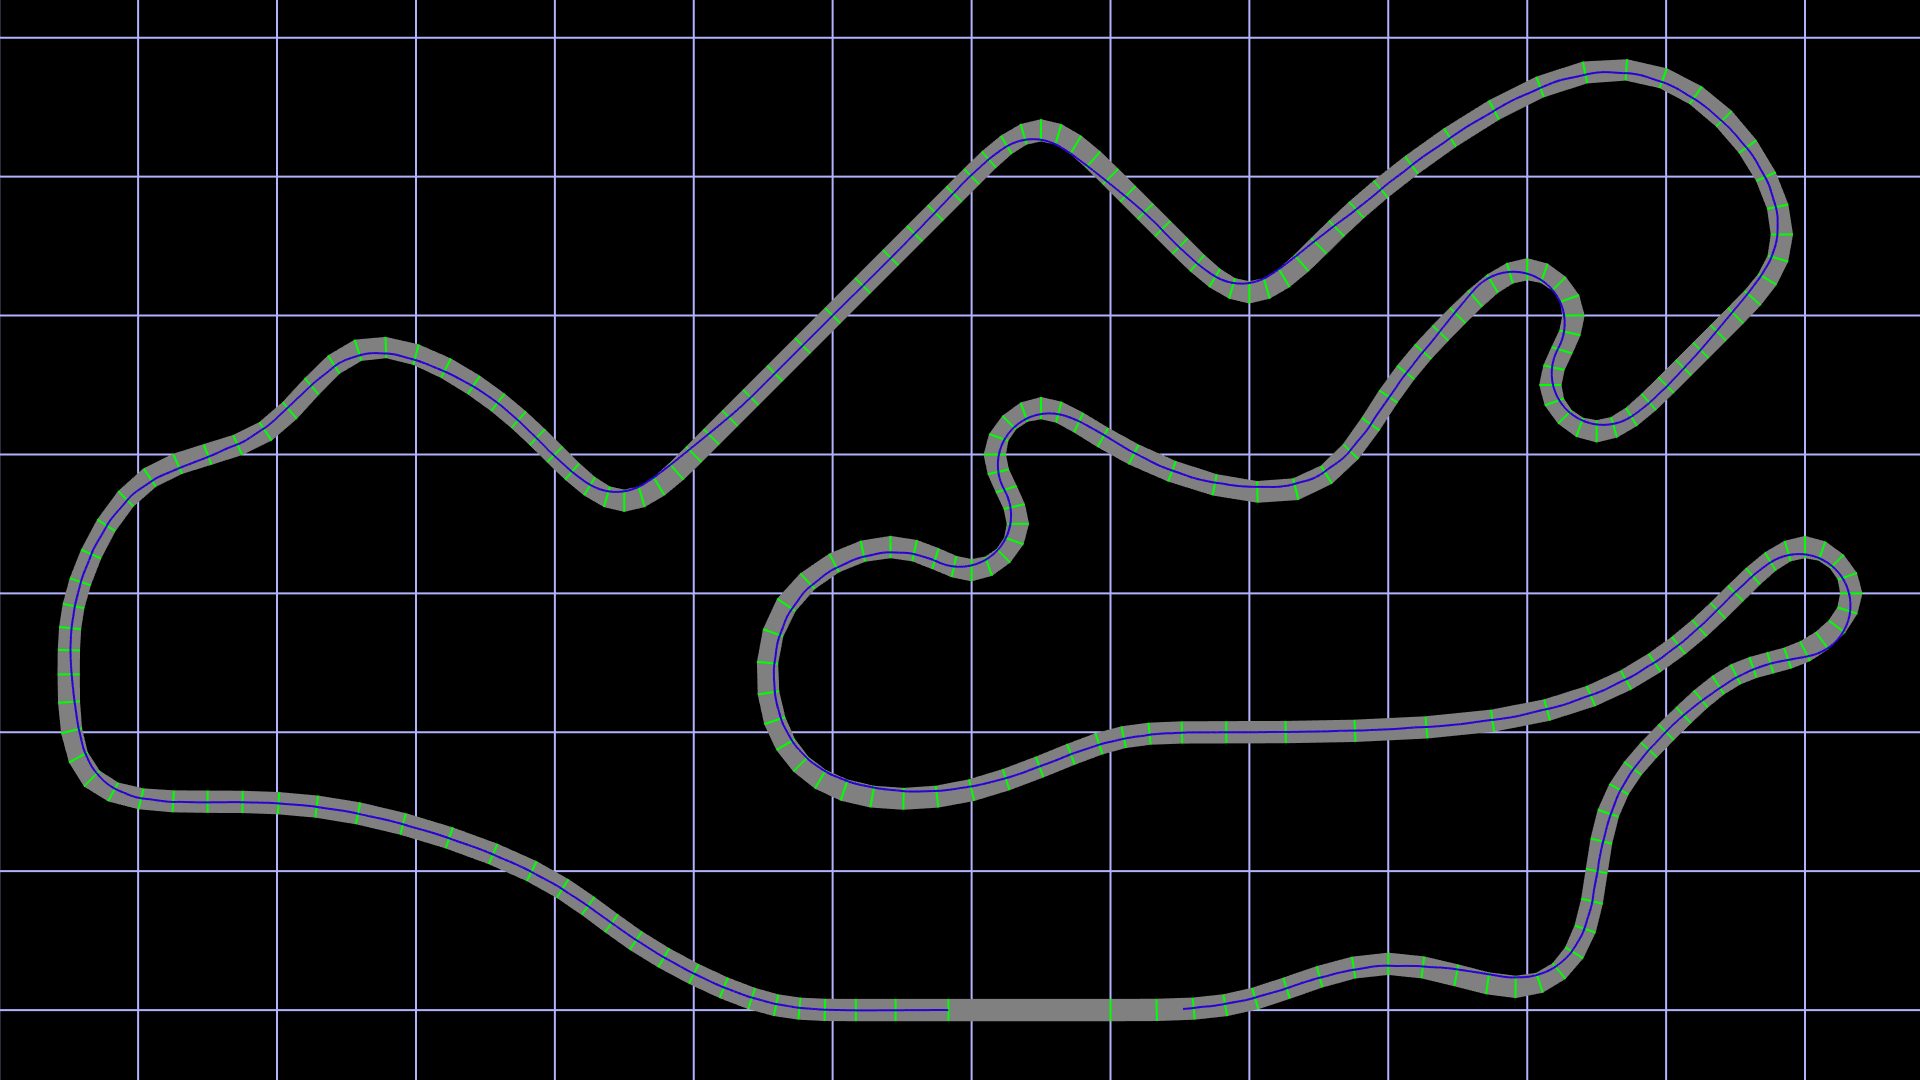
\includegraphics[width=\textwidth]{report/images/fixed_curve_data}
\centering
\caption{Race line showing a clockwise lap performed by the best genome found at the constant speed 12.0 m/s.}
\label{fig:constantspeedline}
\end{figure}

\noindent
At $12.0$ m/s, the system finds an effective behaviour where the AI steers early in the corners as showed in figure \ref{fig:constantspeedline}. At this speed the AI has to push the limits in order to steer through the sharpest corners, as showed in figure \ref{fig:constantspeedsection}. The system managed to complete the whole circuit after $356$ generations. The fastest lap time achieved was $415$ seconds, which was reached after $1225$ generations. Compare this to the $433$ seconds it would take for the car if it was able to travel along the middle line of the circuit at the same speed. The behaviour found at this speed can be considered as close to optimal. The AI behaves effectively in corners. However, it is possible to drive shorter paths through some sections.

\begin{table}[h!] 
  \centering
  \begin{tabular}{rr}
    \toprule
    Generation & Time [s]\\
    \midrule
    $356$  & $417.49$ \\
    $1000$ & $415.70$ \\
    $1225$ & $415.02$ \\
    \bottomrule
  \end{tabular}
  \caption{Showing the best lap times with constant speed $12.0$ m/s, at different stages of the training process.}
  \label{tab:constanttrackdata}
\end{table}

\noindent
At higher speeds, the turning radius became too large to steer through the sharper corners effectively. The AI had to turn very late in the section displayed in figure \ref{fig:constantspeedsection} in order to make it through the second corner. This led to an ineffective behaviour since the AI took late turns in the other corners as well. It also made it less interesting to investigate further, since no effective behaviour was found. 

% Check for longer training sessions
Each of the solutions found showed some typical characteristics. If one solution managed to drive close to the inner side in a sharp corner or positioned itself remarkably before a corner, it also showed that tendency for all other major corners. Similarly, if the AI took late turns in the sharp corners, it took late turns in all corners.

\begin{wrapfigure}{r}{0.5\textwidth}
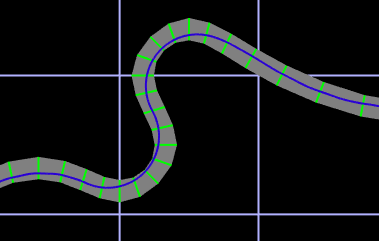
\includegraphics[width=0.5\textwidth]{report/images/constant_speed_section}
\centering
\caption{Race line showing how the best genome found at a constant speed of $12.0$ m/s, drove through the section. The section is approached from the right.}
\label{fig:constantspeedsection}
\vspace{-5pt}
\end{wrapfigure}

%Check for longer training sessions
The recurrent characteristics in the behaviour for a particular solution often had one limitation, that they failed to manage simpler corners as efficient as the tougher ones. Even though near optimal behaviours were observed in the tougher corners, no similarly optimal behaviour was observed in the easier corners. In the simpler sections the system stays close to the middle of the track instead of taking the shorter path along the inner edge. 

%Check for longer training sessions
It seems like the system does not properly learn to distinguish between different levels of corner difficulty. Instead the system finds one behaviour and scales it depending on the situation. Worth noting is that these training sessions only lasted for up to $600$ generations. It is possible that more effective behaviours could be found during longer training sessions. 

\subsection{Shortest Path}
\label{sec:shortest}
The fastest route for a car that moves forward with a constant speed is the shortest one. This means that the only way for a genome to increase its fitness once it completes the circuit is to decrease the distance driven around the track.  

The result show that after the algorithm finds specimens that are able to complete the circuit, the gene pool continues to improve. The path around the circuit is shortened to a great extent. The difference in length of the race line and the middle line of the circuit is significant. 

The optimal behaviour is intuitively to always drive on the inner curves and to drive a straight line between the curves where it has to turn. Small curvature variations should not matter unless the car is required to steer in order to stay on track. 

The car follows the key behaviour aspects, but not to the extent that the path is optimal. We can see that it drives tightly to the inner side for very tight curves, but not for low intensity curves.


% NOTE: Data based on speed_and_control_run_1
\section{Full Control of the Car}
\label{result:fullcontrol}
The base experiment performed, as explained in section \ref{method:baseline}, gives the possibility of controlling speed by controlling the throttle and brakes of the car. The addition of the speed management led to a larger increase in complexity than anticipated. By looking at the results from training sessions, a significant increase in complexity is apparent.

It takes 98 generations until the training process reaches a point where one genome can perform a complete lap. The behaviour observed after 98 generations is one that drives at a constant, slow pace along the track. The car has a fitness value of $5346.8$, which means it travels $5200$ meters in $1110$ seconds, as seen in table \ref{tab:fullcontrol}. Between the corners, the car travels in a straight line along the track. The position at which this line is relative to the tracks mid line changes when the car goes through a corner.

The data shows that the system improves after it manages to complete a lap. The system finds genomes able to drive faster and faster around the circuit. After the system learns to complete the circuit, the rate of improvement is slowed down. As seen in figure \ref{fig:steerspeeddata}, the best genome of each generation increases rapidly until the fitness exceeds fitness of 5200. When this fitness level is reached, the rate of improvement is flattened to a more gradual curve. 

\begin{figure}[h]
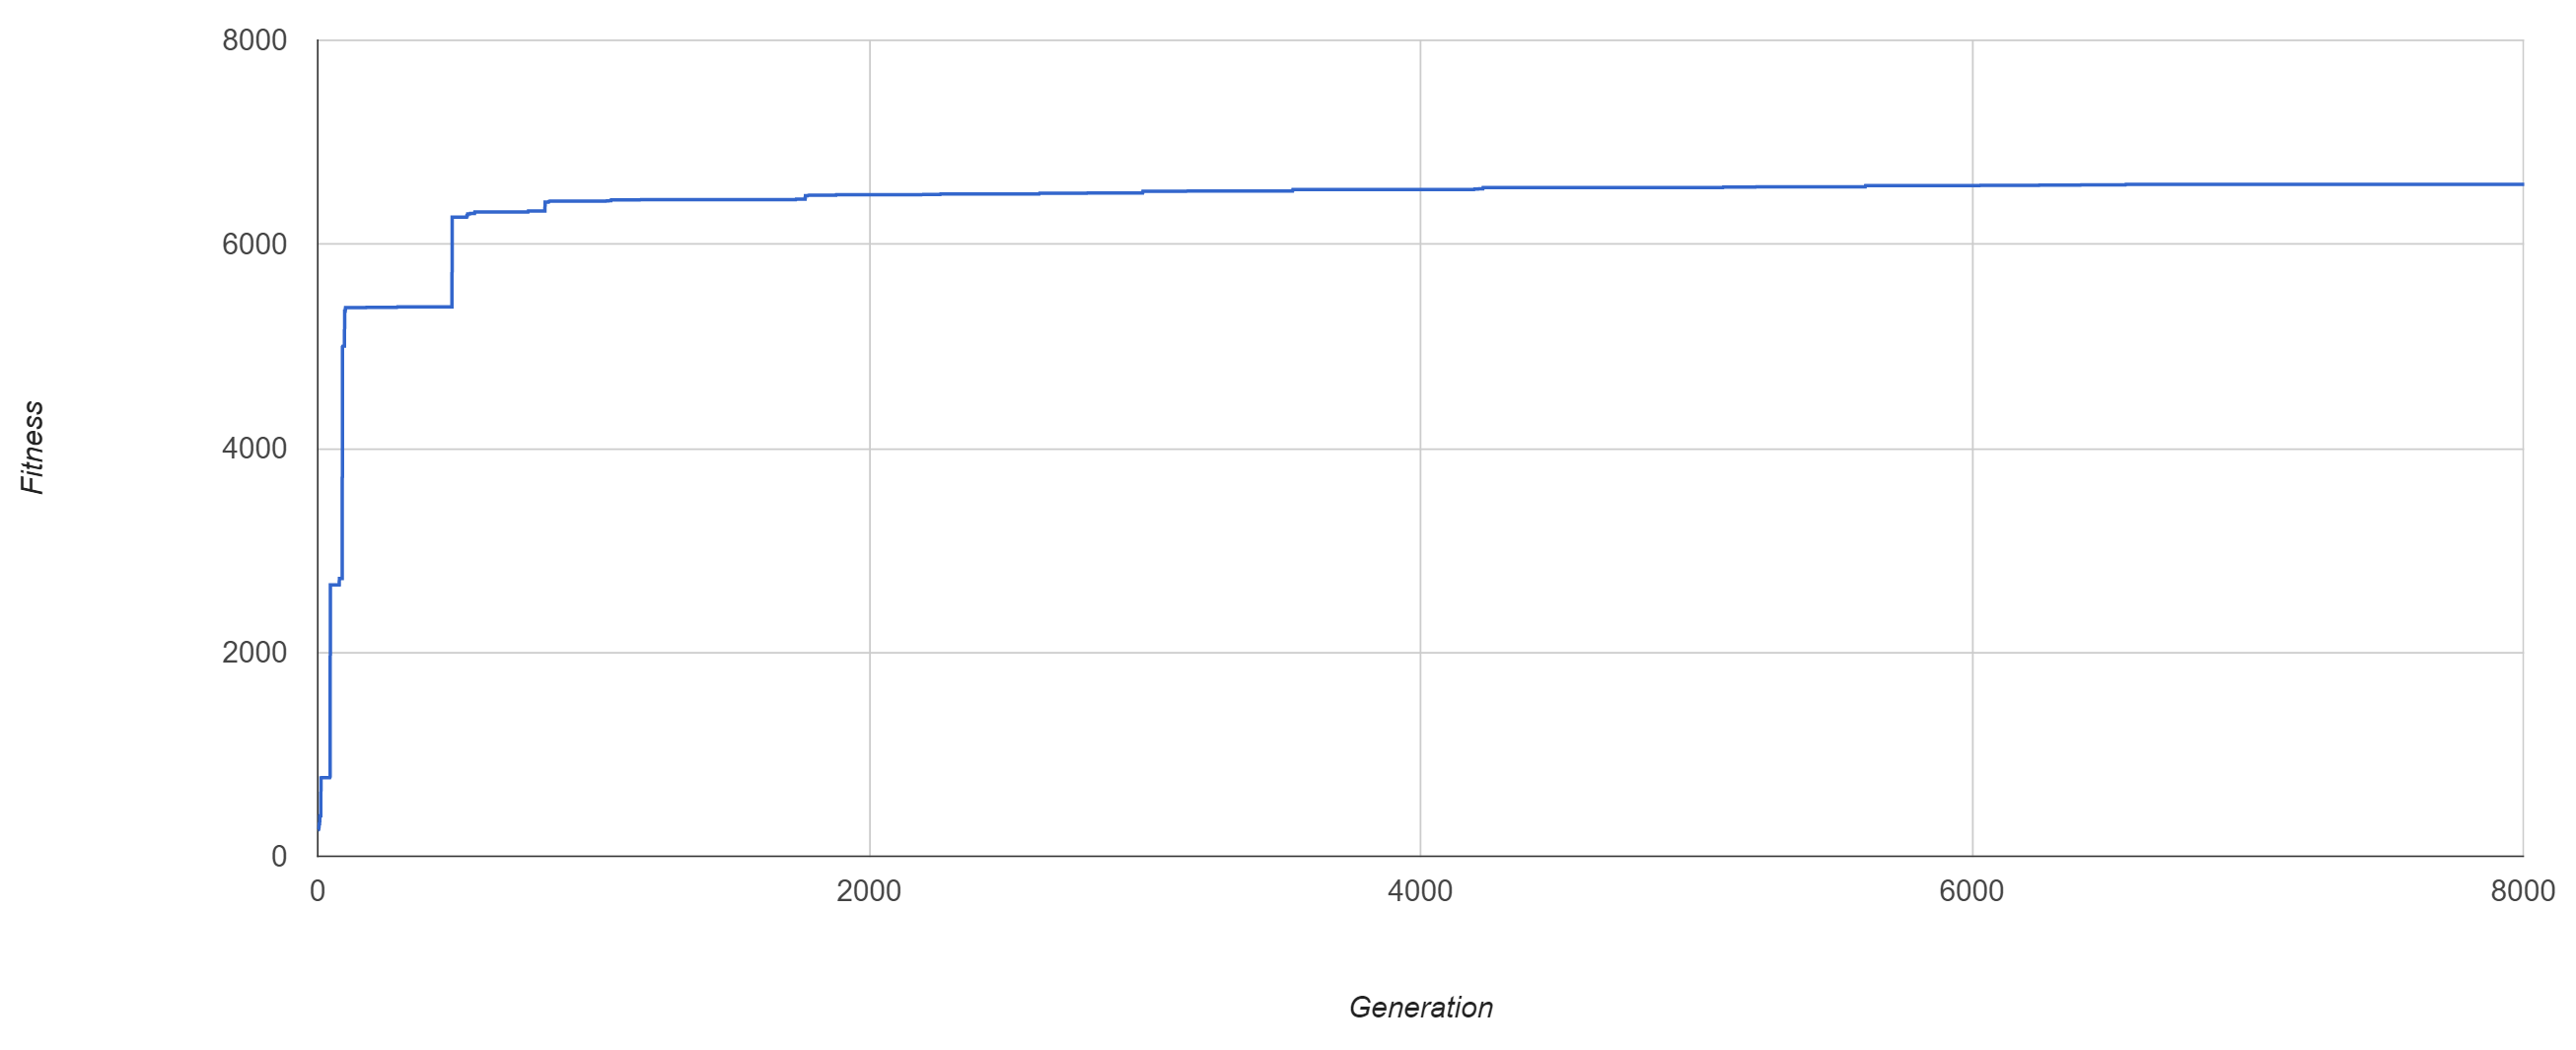
\includegraphics[width=\textwidth]{report/images/graphs/steeringandspeedcontrolrun1}
\centering
\caption{Showing the best fitness of each generation. Note that after 98 generations the fitness value surpasses 5200 as a genome has completed the circuit.}
\label{fig:steerspeeddata}
\end{figure}

\begin{table}[h!] 
  \centering
  \begin{tabular}{rrr}
    \toprule
    Generation & Fitness & Time [s]\\
    \midrule
    $98$ & $5346.81$ & $1110$ \\
    $1000$ & $6423.52$ & $533$ \\
    $8331$ & $6587.56$ & $491$  \\
    \bottomrule
  \end{tabular}
  \caption{Significant results from full control experiment.}
  \label{tab:fullcontrol}
\end{table}

A fitness of $6587.56$ was the highest value that was reached during this experiment. Reaching this fitness value took $8331$ generations, and it corresponds to completing the track in $491$ seconds. Table \ref{tab:fullcontrol} shows that the system manages to lower the lap time significantly. However, the final result as seen in figure \ref{fig:steerspeedline}, is not optimal. Observations from the training process also shows that the path taken by the car at generation $8331$, still resembles the one that was found at generation 98.

\begin{figure}[h]
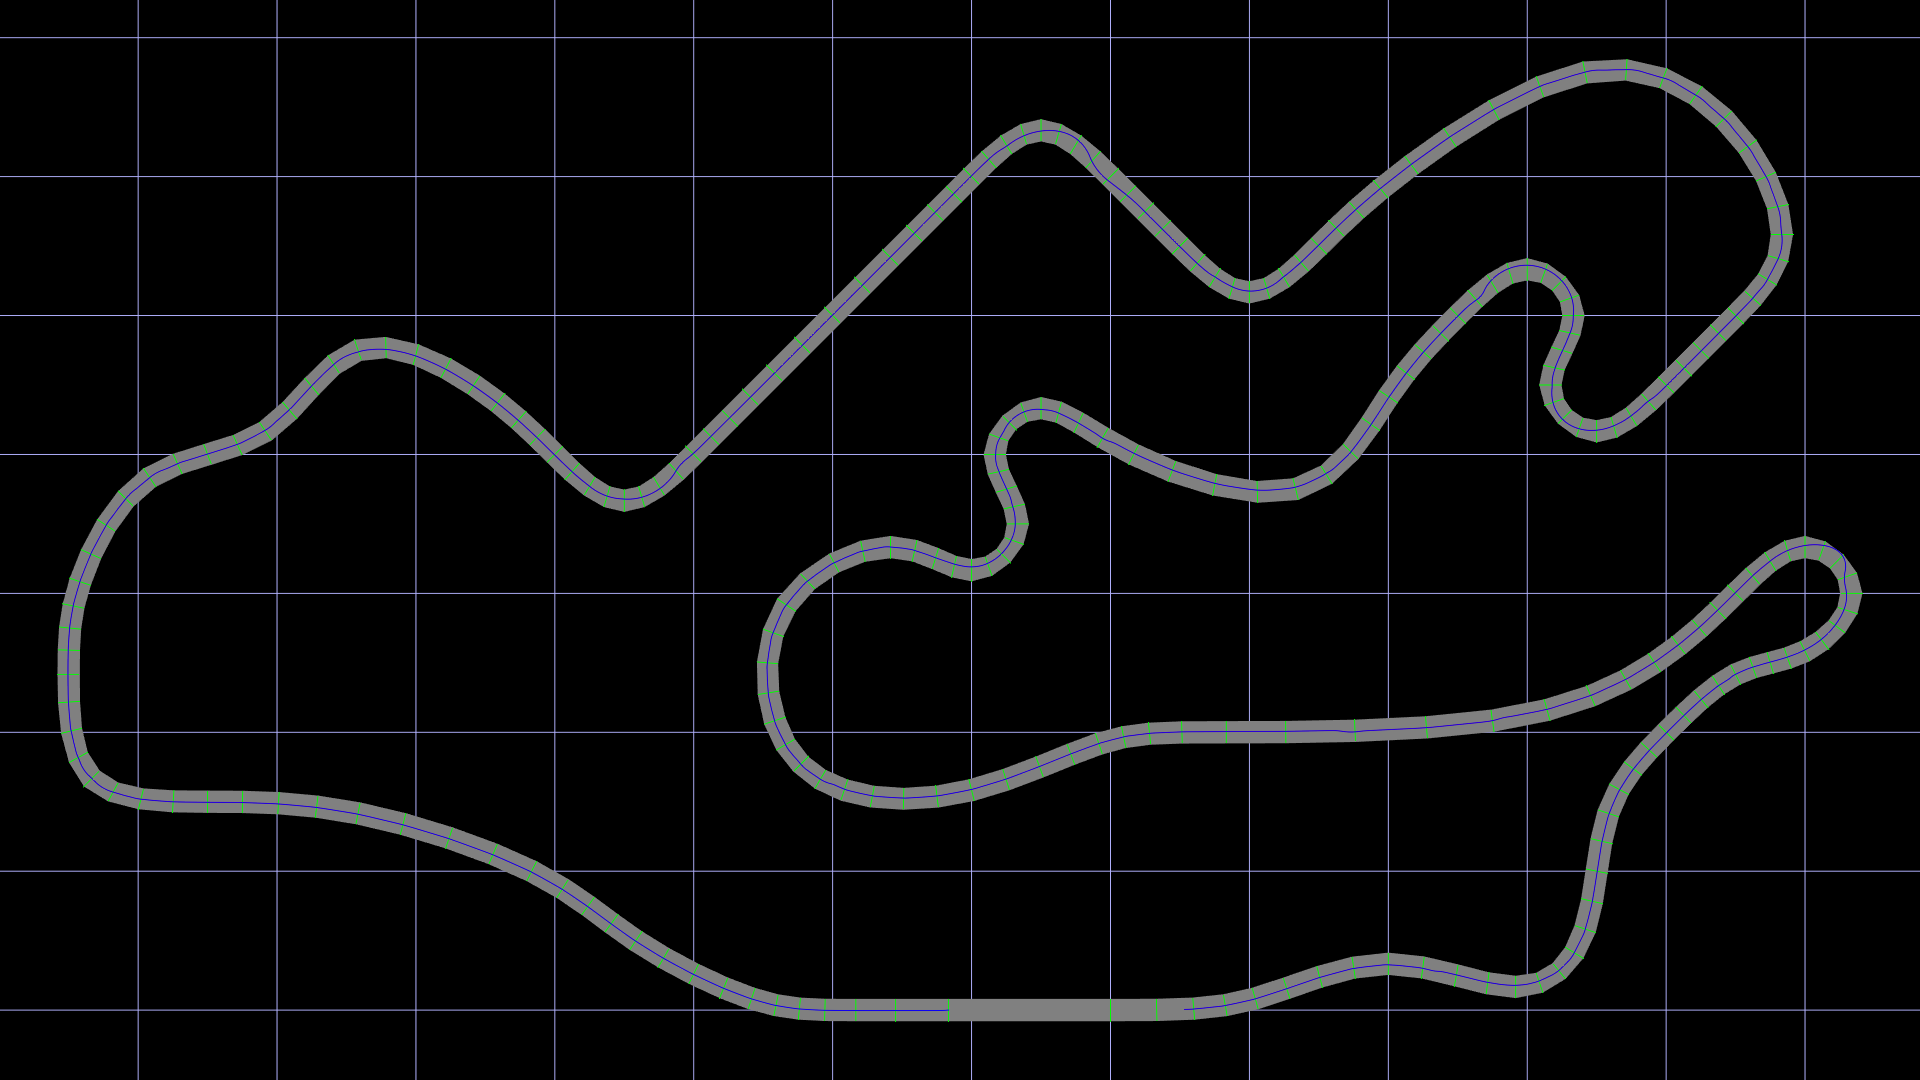
\includegraphics[width=\textwidth]{report/images/normal_generation_6558}
\centering
\caption{Showing a clockwise race line completed by a genome with a fitness value of 6587.56, the best fitness reached in the steer and speed control experiment. The speed of the car is presented by the line colour, with blue as slowest possible speed and red as max speed.}
\label{fig:steerspeedline}
\end{figure}

% - It does not brake/accelerate before/after curves. Why is this? Could the input potentially be modified, such that it is easier for the system to realise what needs to be done? Distance to next curve? 
The decrease in lap time has been observed to be based on two improvements. The first one being the fact that the average speed around the track has increased significantly, and the second one being the increase in acceleration and braking during turns. It has been observed that the car accelerates during the straights and brakes before corners, although very small amounts of acceleration and braking. In order for this behaviour to properly increase the performance of the network, it would have to be more distinguishable.

% The lines that were taken by the best genome can be seen in figure \ref{fig:steerspeedline}. This figure shows that the car does not hold a constant speed throughout the complete track. It can be seen that the car accelerates the slightest at the straights, to use the brake as an action not to hit the wall. This behaviour would need to be more extreme to minimise the time to complete the track; at the current extent, the behaviour is not enough to become faster than the best constant speed genome.
 
Even though the system has the ability to control the brake and throttle in this experiment, it performs worse than the best genome in the constant speed with curvature experiment. After $1000$ generations the constant speed with curvature experiment presents an almost optimal race line for the constant speed. While the best genome in this experiment performs a lap, it does so by simply driving along the track mid line. Although the race lines are significantly different, the lap times are not. Compared to $415$ seconds in constant speed with curvature, this experiment performs a lap by $533$ seconds, which can be seen by comparing generation $1000$ in table \ref{tab:constanttrackdata} and table \ref{tab:fullcontrol}.

Since the system is capable of finding close to optimal race lines when it only controls the steering, as shown in \ref{subsec:fixedspeedcurvature}. It is clear that the performance is altered when the system is given the ability to control the speed. The increase in outputs and possible actions, creates a much more complex environment than in the previous experiments. The increase in complexity leads to a worse overall performance. 

The system never stops positioning the car in the middle of the track, this suggests that the system is over trained before it is allowed to optimise its behaviour for time. Thus, the race line is hard to modify once the system can perform a lap. This initial race line is non-optimal, and thus the maximum speed that is allowed is non-optimal as well. This indicates that it might be beneficial to research the possibility of optimising for time before performing a complete lap.

% Another important aspect/behaviour is that the car is almost in the middle of the track all the time. The line taken by the car only diverges from the middle in the most difficult corners. The constant speed experiment has given a more active line that can be seen at figure \ref{fig:constantspeedline}. The fixed speed line is taking the corners much better, and it can also position the car prior a corner to make a better turn. This is a behaviour that this experiment is missing.

% When the system is given the ability to accelerate and decelerate, it is clear that the performance is altered. The increase in outputs and possible actions, creates a much more complex environment that requires more computation to achieve the same level of results as a system that utilises constant speed. This results in worse performance overall.

\section{Short Track Segment}
\label{result:short}
As hypothesised in section \ref{subsec:shorttracksegment}, the system is able to find more effective behaviours on shorter tracks than on the complete circuit. As shown in figure \ref{fig:short_racelines}, the system drives at a high speed on the straights and brakes in order to steer through the corners. Thus an effective speed management behaviour, which is one of the target behaviour criteria, has been found. However, on these tracks the other criteria, the positioning, is missing. The system does not position the car towards the outer edge or turn early in the corners. 

\begin{figure}[H]
    \centering
    \subfloat[Race line going through the 30-degree corner.]{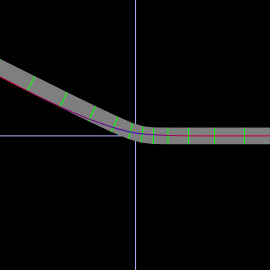
\includegraphics[width=0.28\textwidth]{corner_30_result}}%
    \qquad
    \subfloat[Race line going through the 90-degree corner.]{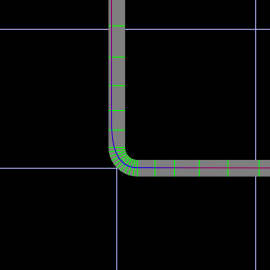
\includegraphics[width=0.28\textwidth]{corner_90_result}}%
    \qquad
    \subfloat[Race line going through the 180-degree corner.]{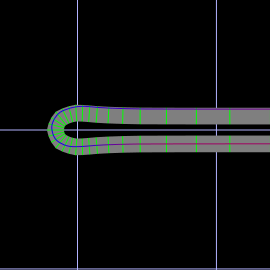
\includegraphics[width=0.28\textwidth]{corner_180_result}}%
    \caption{Race lines through the three corner types. The grey path is the track. The race line goes from red, to blue and back to red. The colour represents the speed of the car, where red is fast and blue is slow. The tracks start in the bottom right corner, and turns right and upwards the figures.}
    \label{fig:short_racelines}
\end{figure}

\begin{table}[H] 
  \centering
  \begin{tabular}{rrr}
    \toprule
    Gen. & Fitness & Time [s]\\
    \midrule
    $10$    & $1067$     & $27.24$  \\
    $1000$   & $1116$    & $20.73$  \\
    $10000$  & $1148$    & $17.20$  \\
    $40000$  & $1164$    & $15.63$  \\
    \bottomrule
  \end{tabular}
  \caption{The progression of fitness and lap times on the track with the 30-degree corner.}
  \label{tab:30deg}
\end{table}

\begin{table}[H] 
  \centering
  \begin{tabular}{rrr}
    \toprule
    Gen. & Fitness & Time [s]\\
    \midrule
    $10$    & $502$     & $-$       \\
    $100$   & $1203$    & $157.34$  \\
    $1000$  & $1835$    & $42.37$   \\
    $8000$  & $2048$    & $25.13$   \\
    \bottomrule
  \end{tabular}
  \caption{The progression of fitness and lap times on the track with the 90-degree corner. No lap times are shown for generations where the track was not completed.}
  \label{tab:90deg}
\end{table}

\begin{table}[H] 
  \centering
  \begin{tabular}{rrr}
            \toprule
            Gen. & Fitness & Time [s]\\
            \midrule
            $10$    & $519$     & $-$       \\
            $100$   & $526$     & $-$       \\
            $200$   & $1456$    & $93.99$   \\
            $1000$  & $1496$    & $86.74$   \\
            $8000$  & $1699$    & $57.13$   \\
            $16000$ & $1882$    & $38.01$   \\
            \bottomrule
        \end{tabular}
  \caption{The progression of fitness and lap times on the hairpin track. No lap times are shown for generations where the track was not completed.}
  \label{tab:180deg}
\end{table}

\noindent
In table \ref{tab:30deg}, \ref{tab:90deg}, and \ref{tab:180deg} the progression of lap times on the short tracks is shown. On all three tracks, the system learns to complete the track in relatively few generations. After that, the lap times are significantly improved. This is mainly due to the AI driving faster and faster on the straights. Overall, the system manages to maintain a significantly higher average pace than on the complete circuit. On the complete circuit, the AI drives with an average speed of approximately $10$ m/s, as seen in table \ref{tab:fullcontrol} on page \ref{tab:fullcontrol}. Compare this with the average speeds of approximately $50$, $37$, and $24$ m/s achieved on the short tracks. 

Even though the system did not find any near perfect behaviours, the results show that the system has a greater ability to optimise for time when training on shorter tracks, than on the complete circuit. One plausible reason behind this is, as mentioned in section \ref{subsec:shorttracksegment}, that it is too hard to change the behaviour of the genomes once they are able to complete the longer circuit. In order to change from a cautious behaviour to a more effective one, the system must learn to accelerate on straights and brake before corners at the same time. Changing only one aspect at a time will most likely lead to a worse behaviour. If a genome is changed to accelerating more it will likely crash in a sharp corner. Likewise, if a genome is changed to braking before corners without accelerating more it will drive slower and thus decrease in fitness.

In order to further improve the behaviour, the system should learn to prioritise the positioning over the braking. Instead of positioning the car effectively and keeping the highest possible speed through the corners, the system disregards the positioning and brakes as much as is needed. How could the training process be designed to promote effective positioning behaviours? Since the system learns to steer effectively in the constant speed experiment, one possible solution is to set a lower bound on the allowed speeds. This would force the system to position the car effectively in order to complete corners. However, deciding which lower speed bound is appropriate is problematic, since it depends on the shape of the track. 


\section{Mirrored Track}
\label{result:mirror}
The mirrored track experiment yielded several interesting results. The test population was trained on the normal circuit until the best specimens managed to complete the circuit in approximately $500$ seconds, which took $3527$ generations. That population was then transferred to and trained on the mirrored track. On the first try, some specimens managed to stay on track for $1800$ metres, which is about a third of the way around the circuit. This shows that at least some of the genomes had some general knowledge about how to drive. However, in the next few generations the migrated population quickly adapted to the new circuit. After only a few generations it managed to complete the circuit. This is, as shown in figure \ref{fig:mirrordata} and table \ref{tab:mirrored}, significantly faster than the control population which took approximately $150$ generations to complete the circuit. 

\begin{figure}[H]
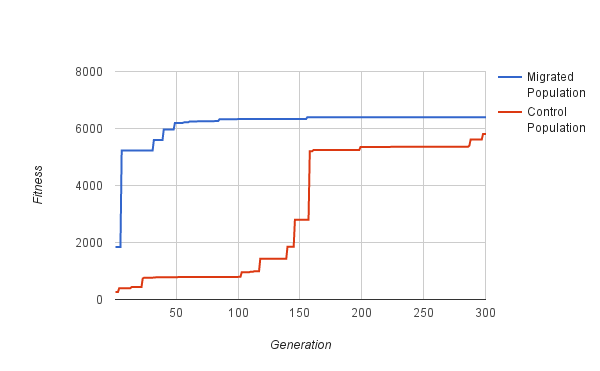
\includegraphics[width=\textwidth]{report/images/graphs/mirror_migration}
\centering
\caption{Showing the fitness progression of the migrated population shown in the thick blue line, and the control population shown in the thin red line. Note that the migrated population in a few generations surpasses a fitness-value of 5200 as a result of completing the circuit.}
\label{fig:mirrordata}
\end{figure}

\noindent
These results show that some of the knowledge acquired on the first track is applicable on the second. The reason may be that the genomes are adapted to similar corners on the first circuit or that the algorithm has found a network structure that is useful in a wide range of situations. In either case, one could argue that in order to find a generalised behaviour the AI should train in an environment where it encounters a wide range of situations, which in the racing domain would be different corners or combinations of consecutive corners. 

\begin{table}[H] 
  \centering
  \begin{tabular}{rrr}
    \toprule
    Generation & Migrated Population Fitness & Control Population Fitness\\
    \midrule
    $1$     & $1839$ & $261$    \\
    $10$    & $5225$ & $397$    \\
    $100$   & $6330$ & $793$    \\
    $200$   & $6397$ & $5355$   \\
    $600$   & $6484$ & $6042$   \\
    \bottomrule
  \end{tabular}
  \caption{Table showing how the migrated population adapted to the mirrored track compared to a control population. Fitness levels over 5200 means that the system has completed the circuit.}
  \label{tab:mirrored}
\end{table}

The extension to the experiment where the migrated population was transferred back to the original circuit once it had adapted also showed interesting results. The population forgets knowledge while adapting to the new environment. This is somewhat expected since the population mutated for 600 generations on the mirrored track, ergo no genomes trained on the original circuit remain in the population. However not all of the knowledge is lost in the process, some knowledge remains. When migrated back to the original track, one specimen manages to stay on the track for circa $2800$ metres, which is slightly past halfway around. After only $5$ generations of adapting back to the original track one specimen manages to complete the circuit, albeit slowly. The adaption to the original circuit is similar in nature to the adaption from the original to the mirrored one. However, one difference is that the adaption rate is slower. As shown in table \ref{tab:mirrored_back}, the migrated population quickly manages to complete the circuit but the improvement of lap times is slow. The migrated population improves slower than when it was trained the first time. One possible reason is that the genomes are larger and thus less flexible. 

\begin{table}[H] 
  \centering
  \begin{tabular}{rrr}
    \toprule
    Generation & Migrated Population Fitness & Original Fitness Progression\\
    \midrule
    $1$     & $2734$ & $261$    \\
    $10$    & $5264$ & $397$    \\
    $100$   & $5264$ & $5347$   \\
    $500$   & $5604$ & $6265$   \\
    \bottomrule
  \end{tabular}
  \caption{Table showing how the migrated population performed when transferred back to the original track. The adaption is compared to how the population progressed when originally trained on the circuit. Fitness levels over 5200 means that the system has completed the circuit.}
  \label{tab:mirrored_back}
\end{table}

These results show that the system is able to find generalised knowledge to some extent. However, the results also show that some knowledge acquired on the original circuit is lost during the training on the mirrored one. One possible reason is that the neural networks become over-fitted to the track they are trained on. This means that the networks have adapted to the track with behaviours that are well suited for that circuit but not in general. The traits responsible for those behaviours are then disabled or changed through mutations when the networks are adapted to the new environment, resulting in a loss of knowledge. One could argue that this loss of knowledge is desired, since the loss of knowledge is a part of adapting to the new environment. However, it is also desirable if the system can learn to solve new problem while it continues to be effective on the earlier problems. If the system stops being evaluated in a specific environment there is no mechanism that preserves knowledge specific to that environment. Thus in order for the system to remember how to solve a problem, the evaluation on that problem must continue. 


\section{Discussion on the Physics Simulation}
The speed held for the experiments was generally low in comparison to the capabilities of the car. The speed achieved, at least for the large track, was about 10 m/s whereas the maximum speed allowed was almost 100 m/s. The constants for the car performance was inspired by formula 1 cars but one mistake was observed late into the experimentation process. The force used for the maximum centripetal force $F_c$ used to turn and rotate the car was notably low, a tenth of the maximum deceleration force. Edmondson (2011) present measurement data for a high performance sports car, for which the maximum lateral acceleration was about double the maximum deceleration. However, it was conceived that the error would only effect the speed for which different optimal behaviours occur, and not the conceptual characteristics.

On the other hand, if the possible speed for which corners could be taken would be larger, the feasible range of speeds would also be larger and that might make it easier for the controller. It might also be worth investigating whether an increased possible speed through the corners, that would close in slightly to the maximum speed, also would make it easier to find a more distinguished behaviour on the straights.

Concerning some of the aspects of physics that were ignored, it probably was a good choice as the results for the simplified physics was not close to optimal. Early experimentation showed that a combined traction budget for the two axis of forces, increased the training times and reduced the performance, understandably as the complexity of the problem increased. This is probably also true for other neglected phenomena.

\section{Discussion on the NEAT Algorithm}
\label{discussion:neat_mechanism}
As described in \ref{theory:neat}, the NEAT algorithm is detached from the actual problem it solves. It is only responsible for the evolutionary process. No analysis of the problem or the simulation results is done in the NEAT system. The only feedback to the system is the fitness value. This makes the algorithm flexible, it is easily adapted to new problems since it is domain agnostic. One might however question how effective it is when solving complex problems.  

The algorithm is not smart. It does not know or understand what aspects of the problem it excels at or what behaviours it is lacking. Therefore, the algorithm has no possibility of applying directed modifications. The progression of the algorithm depends on the availability of an easily reachable better solution. The network topologies are gradually constructed. Each genome is mutated a limited number of times each generation. Thus larger changes to a genome take several generations. In order to produce a successful genome, it is desirable if each gene in the genome is beneficial on its own. If a combination of genes is beneficial but some of the individual genes negatively affect the performance on their own, it is likely that the genes will be discarded before a genome with the combination is found.

If a network performs badly in comparison to the other members of the same species, or if a species performs significantly worse than the other species they will be discarded\cite{stanley:neat}. Additionally, if a species has stagnated, which means that it has not improved for a specified number of generations, it will also be discarded. A third aspect is that worse performing species will have fewer children, thus shrinking in size and in potential diversity. Therefore, the range of time where individual genomes and new innovations can survive is rather well defined. In order to survive it is necessary to improve or at least maintain an above average fitness. Thus it is important for genomes to stay functioning when mutated. Mutations that lead to a significantly worse fitness will fall out of the favourable range and get discarded. It is therefore important that the complexity is gradually increased. If an improvement requires several mutations, NEAT may not be able to find the correct combination of mutations. Thus if NEAT is successful, it likely progressed by a series of small beneficial mutations. 

%[TODO: CHECK RESULT FOR THIS DISCUSSION] 
One example of this is results shown in section \ref{result:fullcontrol}. The genomes learn to drive slowly in order to complete the circuit. Then they will be compared on their lap times, but they may be somewhat locked into the behaviour learnt to complete the circuit. It is possible that there does not exist a path of gradual beneficial mutations to a more aggressive and effective behaviour. The genomes may be stuck in a local fitness maximum. This raised the question of whether it is better to complete the full circuit slowly or only completing a shorter segment but with an effective behaviour

The difficulty of gradual progression may be particularly problematic when achieving behaviours requiring a combination of several components that require each other to be beneficial. If several aspects are required to progress simultaneously, and any of them are missing, it might cause a failure. One example of this can be seen in the full control experiment. If a network changed to drive at a higher speed, but does not change the position of the car accordingly it will likely cause the car to crash. This fact might be one of the reasons as to why some experiments do not perform in optimal ways.

NEAT has proven itself to be useful. We can see in some experiments, e.g. shortest path, that the algorithm is able to find beneficial behaviours that often resemble target characteristics. But it is seldom able to learn all of the smaller details. A behaviour with all of the target characteristics has not been found. Thus it seems like it is hard to find the optimal behaviour using NEAT, due to the problems mentioned above. However, these observations on the key mechanics of the algorithm and the results in our study does not prove that NEAT is unable to find a general and optimal behaviour. Though the observations highlight a structural weakness that cannot be denied. 


\section{Problem Modelling}

In order to achieve the best possible results, it is important to utilise NEAT to its fullest. One important aspect, is how the problem is modelled for the neural network. This includes what information the neural network is provided, and how the results are interpreted by the network.  

The decision process can be divided into two steps. The first is to process and interpret the provided data. The second is to make a decision based on the processed information. It seems like it is beneficial to let the networks focus on the second step. This can be done by only feeding the neural networks with the information required to make good decisions. 


A way to analyse different sets of data is by the information they contain and how relevant it is to the problem. If the data contain noise the training have a more difficult task to learn.

One example is how the system sees the track. The networks could be provided with information describing the track as it is represented in the simulator, a set of three dimensional vectors defining a set of triangles. However, it would have to learn how to interpret and correlate the different data points. The curvature data describes approximately the same thing, which a significantly lower amount of data. The exact coordinates of the triangles are not relevant, the important information is the shape of the track relative to the car.  

To some level, the developer need to do the analysis of what is relevant and good information. If the data get to compact or hard to calculate with, it might get difficult to learn to use it, based on the discussion about multiple goals in section \ref{discussion:neat_mechanism}.

To some extent it might also be important that the values are easily calculable, to make it simpler to find a usage. Several of the input data that was repeatedly used did not provide new information, but was other representations of data already provided. Distance to middle, right and left edge are in a sense analogous as the track in our experiments was uniform in width. The curvature segment data are simply the summation of some of the other data points.

We do often observe that both variants, distances and curvature and their transformations, are used at the same time. It suggests that both variants were usable in the training process, at least at some point. They could have been calculated from the other form of data, but that would have required a more complex network.

\section{NEAT Usability}

The results presented contain both aspects of success and failure. The algorithm manages the control tasks to some degree, but does not achieve the target behaviour, when presented with more complex problems. As discussed in section \ref{discussion:neat_mechanism}, the performance is limited when the steps in which it is required to progress are too large.

As described in section \ref{theory:neat}, NEAT is not an algorithm designed to solve a particular problem. Instead it produces artificial neural networks through neuroevolution. The process is solely controlled by the fitness value. As such, NEAT do not do any particular analysis of the actual problem. 
If NEAT is sufficient to solve a problem, the simplicity makes the algorithm easily implementable as few domain specific processes are needed. It also means that the developer is not required to have as deep domain knowledge, as the algorithm managed to solve the problem on its own. It usually requires more effort and advanced knowledge in order to solve a problem, than it is to know about the problem.

A different approach is as was done in the Stanley project, where not one entity in the system controlled all aspects the driving task \cite{Thrun06}. Different parts of the system were responsible to handle aspects such as perception, planning and steering. Also, in The 2009 Simulated Car Racing Championship the most successful solution had different components in its controller \cite{racingChamp2009}. In a similar way, NEAT might be used with greater success if the particular neural networks are trained for more focused purposes.

%It managed the control task to some degree, but it appears that the usage of NEAT presented uncertainly can solve problems with too much the complexity.
